\section{Background}
    \subsection{Musical Notation}
        In order to understand the task of reading music properly, one must understand a few basic terms.

        \subsubsection{Pitch}
            The pitch of a note is referred to by one of the first 7 letters of the alphabet, i.e. \{C,D,E,F,G,A,B\}.
            In scientific pitch notation, a number from 0 - 8 is added after the letter to indicate which octave the note is in.
            The lowest note possible in this notation, C0, represents a sound with frequency 16.35Hz, and the heighest possible, B8, has a frequency 7902.13Hz.
            A4 (frequency 440Hz) is considered an octave lower than A5 (frequency 880Hz), and an increase in octave represents a doubling of frequency in the sound produced.
        \subsubsection{Duration}
            In addition to pitch, notes also encode information about their duration, or how long the sound should be played. 
            Rests indicate an absence of sound. Both these durations are encoded as in Table \ref{table:notes}

            \begin{table}[h]
                \centering
                \begin{tabular}{| >{\centering\arraybackslash}m{1in} | >{\centering\arraybackslash}m{1in} | >{\centering\arraybackslash}m{1in} |}
                    \hline
                    Name & Note & Rest \\ \hline
                    Semibreve& 
                            
\includegraphics[width=20mm]{./assets/whole.png}
                            &
                            
\includegraphics[width=20mm]{./assets/wholerest.png} \\ \hline
                    Minim& 
                            
\includegraphics[width=20mm]{./assets/half.png}
                            &
                            
\includegraphics[width=20mm]{./assets/halfrest.png} \\ \hline
                    Quaver&
                            
\includegraphics[width=20mm]{./assets/4er.png}
                            &
                            
\includegraphics[width=20mm]{./assets/4errest.png} \\ \hline
                    Semiquaver&
                            
\includegraphics[width=20mm]{./assets/8th.png}
                            &
                            
\includegraphics[width=20mm]{./assets/8threst.png} \\ \hline
                    Crotchet&
                            
\includegraphics[width=20mm]{./assets/16th.png}
                            &
                            
\includegraphics[width=20mm]{./assets/16threst.png} \\ \hline
                \end{tabular}
                \caption{Note and Rest Durations}
                \label{table:notes}
            \end{table}
        \subsubsection{Stave}
            A stave comprises five horizontal lines and four spaces. A note can sit either in a space or on a line, and the height of the note dictates its pitch.
            \begin{figure}[ht!]
                \centering
                
\includegraphics[width=90mm]{./assets/staff.png}
                \caption{The Stave}
                \label{image:stave}
            \end{figure}
        \subsubsection{Clef}
            The pitch of a note on a stave is dependent on the Clef appearing at the start of said stave. There are two types, as below.  
            \begin{figure}[h!]
                \centering
                \begin{subfigure}{0.4\textwidth}
                    \centering
                    
\includegraphics[width=20mm]{./assets/trebleclef.png}
                    \caption{Treble Clef (or G Clef)}
                    \label{image:trebleclef}
                \end{subfigure}
                \begin{subfigure}{0.4\textwidth}
                    \centering
                    
\includegraphics[width=20mm]{./assets/bassclef.png}
                    \caption{Bass Clef (or F Clef)}
                    \label{image:bassclef}
                \end{subfigure}
                \caption{The Clefs}
                \label{image:clefs}
            \end{figure}
        \subsubsection{Bar}
            A bar is a division of time into a number of beats. Each bar is separated by a bar line.
            Separation of music into bars makes music easier to follow.
            \begin{figure}[h!]
                \centering
                
\includegraphics[width=20mm]{./assets/barline.png}
                \caption{Barline}
                \label{image:barline}
            \end{figure}
        \subsubsection{Time Signature}
            Time signature indicates the number of beats in each bar. A time of 4/4 (or C - common time) indicates there should be four crotchets (a.k.a. quarter notes) in each bar; 3/4 indicates there should be 3 crotchets; 2/4 - 2 crotchets; 2/2 - 2 minims etc.
            \begin{figure}[h!]
                \centering
                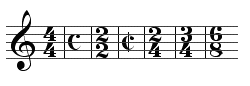
\includegraphics[width=70mm]{./assets/timesignatures.png}
                \caption{Common Time Signatures}
                \label{image:timesignatures}
            \end{figure}
        \subsubsection{Beams}
        Beams link together two or more consecutive quarter notes (or smaller divisions) to indicate a rythmic or melodic grouping, e.g. multiple notes for a single sung syllable. 
            \begin{figure}[h!]
                \centering
                
\includegraphics[width=20mm]{./assets/beam.png}
                \caption{Beamed Notes}
                \label{image:beam}
            \end{figure}
        \subsubsection{Dots}
            A dot after a note indicates that the note should be played for 1.5x normal duration, e.g. a dotted minim has the same duration value as a minim and a crotchet combined.
            \begin{figure}[h!]
                \centering
                
\includegraphics[width=20mm]{./assets/dotted.png}
                \caption{Dotted Note}
                \label{image:dotted}
            \end{figure}
        \subsubsection{Accidentals}
            Accidentals change the pitch of the notes they are associated with. A sharp increases the pitch by a semitone (the difference between a B and a C). A flat decreases the pitch by a semitone. A natural accidental nullifies any changes to the pitch.
            \begin{figure}[h!]
                \centering
                \begin{subfigure}{0.3\textwidth}
                    \centering
                    
\includegraphics[width=20mm]{./assets/sharp.png}
                    \caption{Sharp}
                    \label{image:sharp}
                \end{subfigure}
                \begin{subfigure}{0.3\textwidth}
                    \centering
                    
\includegraphics[width=20mm]{./assets/flat.png}
                    \caption{Flat}
                    \label{image:flat}
                \end{subfigure}
                \begin{subfigure}{0.3\textwidth}
                    \centering
                    
\includegraphics[width=20mm]{./assets/natural.png}
                    \caption{Natural}
                    \label{image:natural}
                \end{subfigure}
                \caption{Accidentals}
                \label{image:accidentals}
            \end{figure}

    \subsection{Computer Vision and OMR}
        \subsubsection{OpenCV}
            OpenCV\cite{OpenCV} is an open source Computer Vision library. It is written in Native C++. We are using OpenCV4Android\cite{OpenCV4Android} which allows us to work completely in Java. This then calls the original C++ implementation through the Java Native Interface (JNI)\cite{JNI}. We have used the OpenCV library for two things: firstly to implement a camera, secondly to process the images.

        \subsubsection{Representing Images}

Bitmaps are perhaps the simplest method of representing an image. A bitmap is simply a 1 to 1 mapping for the value of each pixel in an image. Usually, bitmaps have multiple ‘channels’ to store multiple values for each pixel. The convention for digital photographs is to have 3 channels, one for Red, Blue, Green. This is known as the RGB format.

However, many existing computer vision techniques work only on a single grayscale channel, or even on a binary (black and white) image. Therefore, pre-processing is sometimes required.

In this project we have used the Android implementation of Bitmaps\cite{Bitmap}.

        \subsubsection{Grayscale Conversion} \label{sec:grayscale}

Converting a full color image to grayscale is a relatively simple operation, for each pixel in the image you simply find the average value of each color channel. The new image can be represented by a single channel, which reduces the memory requirements 3-fold. Obviously, some information will be lost in this process as many different colors will map to the same grayscale value. However, sheet music does not assign any semantic meaning to different colors and so this is not an issue for our project.

        \subsubsection{Image Thresholding} \label{sec:threshold}

Converting a grayscale image to a binary (black and white) image is also a simple process. A threshold is chosen and all intensity values below the threshold are set to black while all values above it are set to white. The \lq intensity\rq of a grasycale pixel simple refers to that pixels value from 0-255. However, deciding on this threshold value is a non-trivial problem and is explored further in our implementation.   
\[ f(i,t) = \left\{ 
  \begin{array}{l l}
    255 & \quad \text{if } i \leq  t\\
    0   & \quad \text{otherwise}
  \end{array} \right.\]

        \subsubsection{Erosion and Dilation} \label{sec:erosion}

When you want to detect a specific feature of an image it can often help to emphasise that feature through image processing. Erosion and dilation are two common ways in which this might be done.

Eroding an image means to expand the black areas of the image, while dilating means to expand the white areas of the image. This has a wide variety of applications such as removing noise, filling small gaps and highlighting important features.
            \begin{figure}[ht!]
                \centering
                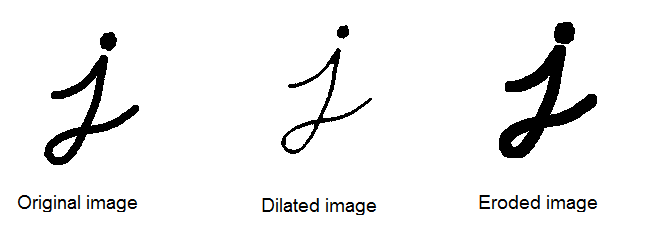
\includegraphics[width=90mm]{./assets/dilated.png}
                \caption{Erosion/Dilation}
                \label{image:dilationerosion}
            \end{figure}

The algorithm that does this performs an operation on each pixel in the image using a supplied kernel. It performs the calculations depending on the surrounding pixels intensity as well as the kernel values, and returns a value that will state whether the given pixel becomes black or white. Intuitively, the kernel can be thought of as a matrix represents the area around each pixel to look into, centred on the pixel of interest. A change in the shape or size of the kernel can lead to totally different processing effects. The effect will also depend on the quality of the image and the lighting conditions.

It is important to note that each eroding/dilating operation requires some thinking and testing about its kernel shape and size.

\subsubsection{Projections} \label{sec:projections}

There are two basic types of projections: horizontal and vertical. A horizontal projection performs an operation on each row of the image. You end up with a new image of width 1 and the same height as the original image. In our case, we always average the values in the grayscale image channel.
Similarly, a vertical projection performs the same operation on columns and outputs a new image of height 1 and the same width as the original image. The operation we use is also the average of the intensity values.

\begin{figure}[h!]
	\centering
	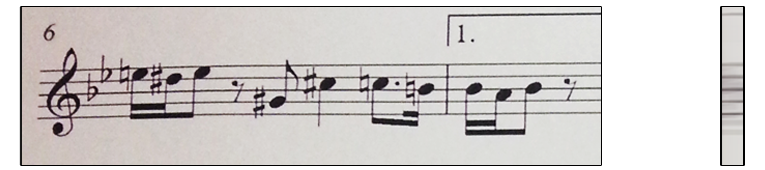
\includegraphics[width=1\textwidth]{./assets/projectionBackground.png}
	\caption{An example image with its corresponding horizontal projection}
	\label{image:projectionBackground}
\end{figure}

\subsubsection{Contours} \label{sec:contour}

A contour is a boundary between two areas of different color in an image. On a black and white image, this will separate the black from the white areas. The built-in method \verb!findContours!\cite{findContours} in the OpenCV library finds all contours in a given image, returned as a list of matrices, by following a complex algorithm that is outside the scope of this document. The contour can then be processed to find useful information such as its center of gravity.

Intuitively, the center of gravity of a shape represents the point that a human would call its ‘center’. For a highly symmetric shape, like a circle or star, this will be located in the geometric center of the shape. For an uneven shape, like a hammer, the center of gravity may be quite far from the geometric center of that shape.

We can find the center of gravity of a contour using the following formulae:
\begin{equation}
    x = \frac{ m_{1,0}}{m_{0,0}}
\end{equation}
\begin{equation}
    y = \frac{m_{0,1}}{m_{0,0}}
\end{equation}
where $m_{i,j}$ denotes the $i$th moment on $x$ and $j$th on $y$



\subsubsection{Hough Transforms} \label{sec:hough}

Hough transformations are feature-extraction techniques that work by transforming the image into a new mathematical space where the desired feature is highlighted. The two most commonly used Hough transformations are Hough lines and Hough circles, which detect straight line segments and circles respectively.

The Hough lines transformation highlights the location, direction and length of all lines on that image. Points above a given threshold are then extracted from this image and converted into line segments.

It can be very useful for detecting long, thick lines in a source image but it does not perform well with short or thin lines. Also, because the algorithm is probabilistic, small lines that are next to a larger line may be considered noise and be ignored. Also, if a line is even slightly bent then it will register as several smaller lines or possibly not be detected at all. Finally, the algorithm is very slow as it checks every pixel in the
image, which is a serious problem for an Android device as it has little processing power.

Hough circles is a similar algorithm that detects circles in an image. It has similar strengths and weaknesses to Hough lines.

\subsubsection{Template Matching} \label{sec:template}

Template matching is a technique for detecting complex, arbitrary patterns in a source image. It searches the source image for areas that best match a given ‘template’ image.

It works by performing the following check on each pixel of the source image. Starting from that pixel, we select an area of the source image of equal size to our template. Then, we can check how well that area matches the template by comparing each pixel to its corresponding pixel on the template and then combining these results. 

Once we have done this for each pixel in our source image, we can extract all the matches that are above a certain threshold. While doing this, we must consider that if one pixel is a good match, the pixels surrounding it are likely to be good matches too and so we require a minimum distance between any 2 matches.
    
            \begin{figure}[h!]
                \centering
                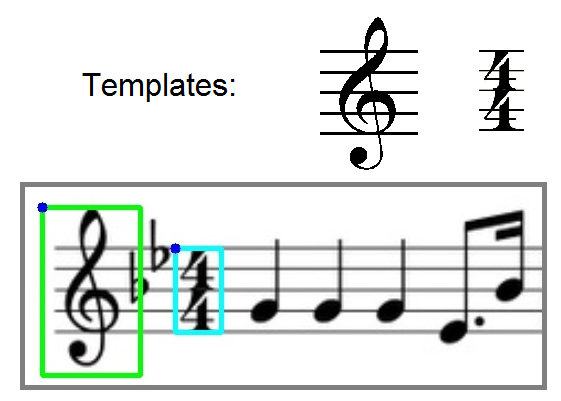
\includegraphics[width=90mm]{./assets/templatematch.png}
                \caption{Best matches for 2 different templates}
                \label{image:templatematch}
            \end{figure}

Another important consideration is the selection of a pixel comparison method. It is perhaps counter-intuitive, but it is not enough to simply check which method gives the best matches. Rather, we need to find the method that gives the most distinct results, ie. the greatest difference between the least accurate positive match and the most accurate negative match. This is because the method uses a threshold value to determine
which values constitute a match, and this threshold must fit within our tolerance gap.

As expected from looking through the literature, we found that the ‘correlation-coefficient’ approach gave us the best results and we used it throughout the project.  
It is given by the following equation:
\begin{equation}
	C(x,y) = \sum_{x'y'} T'(x',y') I(x+x',y+y')
\end{equation}

where $x'$, $y'$ sum over the dimensions of the template image, and $T(x,y)$ and $I(x,y)$ return the intensity values found at those coordinates in the template and source image respectively.
The major advantage of template matching is its ability to match an arbitrary pattern. While most other algorithms are highly specialised to detect a single feature like straight lines, template matching can find virtually any distinctive pattern in an image. However, this also presents its greatest drawback: it searches for a very specific pattern and is therefore very intolerant to slight variations in this pattern. It
is also slow as it operates on each pixel in the image.

Another drawback of template matching is that there is no built-in method to extract more than one result. While there exists a method, \verb!minMaxLoc! in the org.opencv.Core package, that returns the location and value of the best result there is no trivial way to extract any further results. The way we worked around it was by zeroing all the pixels in a specified area around the best result and calling \verb!minMaxLoc! again until the associated value reached a certain threshold. This threshold has to be fine tuned for each feature we want to template match.

For best results the technique should be used on a very specific and distinctive pattern. It should typically be used when more specialised solutions are not applicable.

    \subsection{Android} \label{sec:android}
When working with Android the provided paradigm for managing the flow of your application is through the use of Activities. As described in the android developer guide:

\begin{quote} 'An activity is a single, focused thing that the user can do. Almost all activities interact with the user, so the Activity class takes care of creating a window for you in which you can place your UI' - \href{http://developer.android.com/reference/android/app/Activity.html}{Android Reference}
\end{quote}  

The app starts with a main activity which can then cause other activities to be started to do different tasks. Activities are kept on the ‘back stack’, which operates on the normal first in last out (FILO) order. When a new activity is started it gets added to this ‘back stack’, when that activity finishes we go back to the activity before, similarly when the device back button is pressed. This means that by using
activities in our app it enables the user to move through the app as they are used to using the back button as usual. Also if the app is minimised and then reopened it will retain its place.

